\documentclass[11pt, twoside, a4paper, openright]{report}

\usepackage{../source/util}
\graphicspath{ {../img/intro/} }

\begin{document}
\chapter{Introduction à la cosmologie}

Ce premier chapitre a pour but de présenter la cosmologie moderne et d'expliquer brièvement sa construction au fil du dernier siècle. L'idée est de donner une vue d'ensemble du paradigme actuel, tout en détaillant davantage les points clés nécessaires à ce manuscript. Pour une étude approfondie de la cosmologie moderne, nous referons le lecteur aux ouvrages suivants : \cite{CITE}. 

\section{Qu'est-ce que la cosmologie ?}
Le terme cosmogonie (du grec \emph{cosmo-} : monde ; \emph{gon-} : engendrer) désigne une conception et tentative d'explication de la naissance du monde, et parfois de l'Homme. Il existe une grand nombre de cosmogonie, três souvent d'origines religieuses. Nous pouvons citer par exemple la cosmogonie hindoue, dans laquelle le monde est vu comme un cycle : le dieu Brahma crée le monde lorsqu'il se réveille, et le dédruit lorsqu'il s'endort. Notre univers correspond ainsi à une journée de Brahma, débutant lorsque Brahma ouvre les yeux et prenant fin lorsqu'il les referme. Le monde suit ainsi une suite de créations et de destructions.
Nous pouvons aussi citer la cosmogonie abrahamique, décrite dans la Genèse. Cette cosmogonie est commune au judaïsme et au christianisme, et est reprise dans le coran. Dans cette cosmogonie, le dieu créateur, intemporel, conçut le monde en 7 jours. Il commença par créer la lumière le premier jour. Il termina par créer l'Homme à son image le sixième jour, puis se reposa le dernier jour.
\begin{figure}
  \centering
  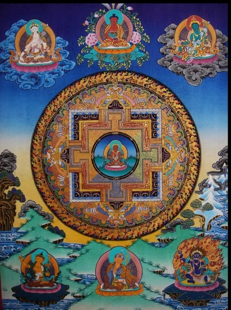
\includegraphics[scale=1]{cosmohindoue.png}
  \hspace{3cm}
  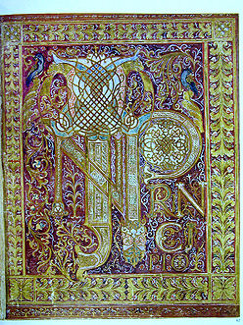
\includegraphics[scale=1]{genese.png}
  \caption{Gauche : illustration artistique de la cosmologie hindoue. Droite : couverture du livre de la Genèse, Bible de Staint-Paul-hors-des-Murs, vers 870.}
  \label{fig:cosmohindoue}
\end{figure}

Nous pourrions passer la totalité de ce manuscript à décrire diverses cosmogonies. Mais celle qui nous intéresse et que nous allons détailler ici est la cosmogonie scientifique : la \emph{cosmologie}. La cosmologie est donc l'étude de l'univers, son origine, ses constituants et son devenir, dans le cadre de la méthode scientifique. Même si aujourd'hui la cosmologie fait consensus en ce qui concerne la compréhension de l'univers, cela n'a pas toujours été le cas. Pendant longtemps les croyances religieuses ont dominé, allant jusqu'à limiter les avancées scientifiques. Il faut attendre le \textsc{XVI}\ieme~siècle pour que Copernic propose le modèle héliocentrique et s'oppose ainsi au modèle géocentrique soutenu par l'église et les savants de l'époque. Par la suite, les observations de Galilée, les travaux de Kepler ainsi que l'émancipation des dogmes religieux ont permis au modèle héliocentrique, basé sur les lois de Kepler, de s'imposer. Cela a aussi permis à Newton de proposer sa théorie de la gravitation peu de temps après. Cette période marque la naissance de la physique et de la cosmologie.

Jusqu'au \textsc{XIX}\ieme~siècle, le modèle héliocentrique décrivant l'univers comme étant notre système solaire fait consensus. Puis émerge l'idée que les étoiles sont d'autres systèmes solaires, notament grace aux premières mesures de distance d'étoiles proches\footnote{Par exemple la mesure de la distance de 61 Cygni par Bessel en 1838. \#prov https://www.universalis.fr/encyclopedie/premiere-determination-de-la-distance-d-une-etoile/}. L'idée de galaxie, un système rassemblant une multitude de systèmes solaires, fait aussi sont apparition, nous conduisant vers un paradigme de moins en moins anthropocentrique.

\paragraph{} La cosmologie moderne naît réellement au début du \textsc{XX}\ieme~siècle. En 1915, Einstein propose sa théorie de la gravitation : la \emph{relativité générale}. Elle offre une vision radicalement différente de la théorie bien établie de Newton. La gravitation n'est plus vu comme une force instantannée entre les corps massifs mais comme une déformation de l'espace temps se propageant à la vitesse de la lumière. La théorie d'Einstein explique avec succès le décalage du périhélie de Mercure, jusque là incompris. Puis en 1919 lors d'une éclipse de Soleil, la déviation de la lumière par un corps massif, prédiction directe de la relativité générale et non présente dans la théorie de Newton, est observée. Ceci assoit au sein de la communauté scientifique la théorie d'Einstein en tant que nouvelle théorie de la gravitation.

Par ailleurs, la cosmologie observationnelle connaît des avancées remarquables, notament grace à Edwin Hubble qui observe le décalage vers le rouge\footnote{voir explication du redshift section \#prov:ref} du spectre d'objets lointains, dû à leur éloignement. Il comprend aussi que les objets étendus, jusque là interpretés comme des nuages de poussière et de gas et appelés nébuleuses, sont d'autres galaxies semblables à la nôtre. Parallèlement, Alexandre Friedmann résout en 1922 les équations d'Einstein de la relativité générale et trouve une solution d'univers en expansion, qui contraste avec l'idée d'un univers statique et éternel jusque là ancrée dans les esprits. Enfin, Georges Lemaître effectue le lien entre tous ces éléments. En 1927, il publie un papier explicant que l'éloignement des galaxies et le décalage vers le rouge de leur spectre pouvait être expliqué par une théorie d'univers en expension, et donne la première estimation de la constante de Hubble\footnote{Constante reliant proportionnellement la vitesse d'éloignement des galaxies à leur distance, voir \#prov:ref}. En 1929, Edwin Hubble publie son célèbre papier, exposant la loi de Hubble et favorisant très fortement le modèle d'univers en expansion.

\paragraph{} Ces 15 années très fertiles pour la cosmologie ont démocratisé l'idée d'un univers en expansion. Si certain s'y oppose fermement, d'autres s'y intéressent et étudient en détail les conséquences de ces modèles théoriques. Si l'univers est en expansion, c'est qu'il a été dans le passé plus petit qu'il ne l'est aujourd'hui. L'étude des solutions aux équations d'Einstein montre que l'expansion dilue la matière dans l'univers, et conduit à son refroidissement. L'univers était donc plus chaud et plus dense dans le passé. Ces points conduisent à nommer ces classes de solutions \emph{hot big bang models}, ou modèles de big bang en français, symbolisant l'idée qu'aussi loin que nous puissions remonter, l'univers fût un point infiniment chaud et dense.


\bibliographystyle{unsrt}
\bibliography{../source/biblio}

\end{document}
